\documentclass[12pt, onecolumn, letterpaper, oneside]{book}

\usepackage{authblk}
\usepackage[autostyle]{csquotes}
\usepackage{amsmath}
\usepackage{graphicx}
\usepackage{hyperref}
\usepackage[sc]{titlesec}
\usepackage{titlepic}

\usepackage[square,numbers,sectionbib]{natbib}
\usepackage[sectionbib]{chapterbib}
\usepackage{titlesec}
\usepackage{indentfirst}

\usepackage{tikz}
\usepackage{rotating}

\usepackage{wasysym}

\titleformat{\chapter}[display]
  {\rmfamily\scshape\bfseries}{}{0pt}{\Large}
\titleformat{\section}[display]
  {\scshape}{}{0pt}{\large}
  
 \usepackage{scrextend}
 \interfootnotelinepenalty=10000

\usepackage{fancyvrb}
\usepackage{suffix}

\newcommand\chapterauthor[1]{\authortoc{#1}\printchapterauthor{#1}}
\WithSuffix\newcommand\chapterauthor*[1]{\printchapterauthor{#1}}

\usepackage{fancyhdr}
 
\pagestyle{fancy}
\renewcommand{\chaptermark}[1]{\markboth{}{\uppercase{\itshape #1}}}
\fancyhf{}
\fancyhead[L]{\rightmark}
\fancyhead[R]{\thepage}
\renewcommand{\headrulewidth}{0pt}
 
 \renewcommand\thefigure{\arabic{figure}}

\makeatletter
\newcommand{\printchapterauthor}[1]{%
  {\parindent0pt\vspace*{-25pt}%
  \linespread{1.1}\large\scshape#1%
  \par\nobreak\vspace*{35pt}}
  \@afterheading%
}
\newcommand{\authortoc}[1]{%
  \addtocontents{toc}{\vskip-10pt}%
  \addtocontents{toc}{%
    \protect\contentsline{chapter}%
    {\hskip1.3em\mdseries\scshape\protect\scriptsize#1}{}{}}
  \addtocontents{toc}{\vskip5pt}%
}
\makeatother

\title{Anarchao Discordia\\
		\vspace{1\baselineskip}
		\large{Vol. I}
		%\large \textit{a journal of anarchist ideas}\\	
		%\normalsize ``There is no governor present anywhere.'' --- Chuang Tzu
		}
\date{July, 2018\\
		 Confusion, YOLD 3184}
\author{Editor: Griffensteed the 5$^\text{lth}$\\
			'Patafizikhood of Eris Esoteric\\}
\titlepic{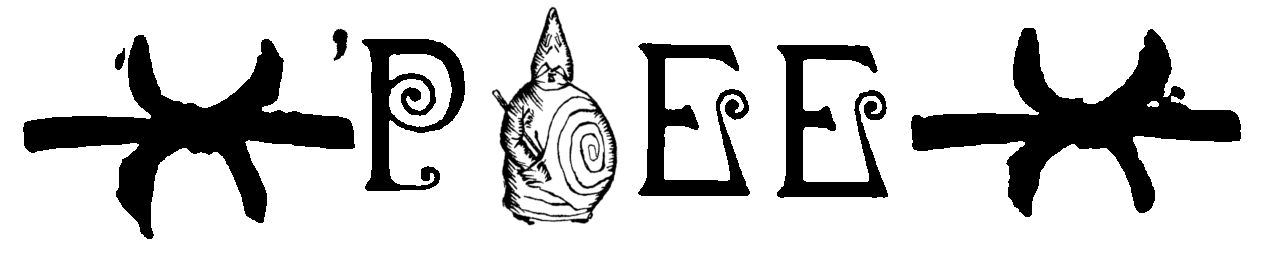
\includegraphics[scale=0.3]{./img/poee.png}}


\fancyfoot[L]{Confusion, YOLD 3184}
\fancyfoot[R]{Anarchao Discordia}

%\setlength\parindent{0pt}
    \setlength{\columnsep}{1cm}

\begin{document}
\sloppy

\maketitle

\tableofcontents

\chapter*{Notes}
\begin{verbatim}
The (re)discovery of anarchism through Discordia.
The (re)discovery of Discordia through anarchism.           
\end{verbatim}

\begin{center}
\emph{Dysnomia (Anarchy), Daughter of Eris.}\\
\end{center}

Discordianism and Anarchy always felt to me intrinsically linked by their origins, their ideologies, their authors, their vessels, and their methods. After looking around, it appeared to me that since 1990 with the end of \emph{No Governor}, edited by Robert Shea, no other publication reunited this mother and daughter, and I felt a need to reignite that flame.\\
I felt a need to (re)discover old and new anarchist and discordian thinkers and compile their thoughts and opinions; to see how old ideas from different parts of our world still hold firmly in our current society; to express new ideas about the new openings and new dangers arising for which anarchists and discordians must prepare.\\

\begin{center}
Anarchao Discordia\\
\end{center}

This first installment of \emph{Anarchao Discordia} mostly focuses on setting the basis of what the readers can expect in the future. It also aims at ``priming the pump" with some great articles from famous authors, laying the foundations of anarcho-discordianism, such as Robert Anton Wilson \& Robert Shea (p.4) and Gregory Hill (p.21); an excellent interview of Cornelius Castoriadis (translated from French) about freedom and the insignificance of modern politics (p.23), considered by Castoriadis as a ``message in a bottle" for future generation (i.e., us); a proto-discordian manifesto on music by John Cage (p.30); and an article, by me, about ``mathematical conspiracy theory" applied to the separation of powers in representative democracy (p.12).\\

If you feel interested in this project, similarly to \emph{No Governor}, \emph{Anarchao Discordia} needs three forms of help:
\begin{enumerate}
\item It needs to be read. Words, thoughts and ideas can only live if they reach minds. \emph{Anarchao Discordia} is published under a GNU GPLv3 licence, so please, feel \textsc{free} to share and distribute as you please.
\item It needs articles. If you would like to express your opinion and ideas on society, your experience, your strategies and solutions to solve modern plagues, your views on current events, etc. from a anarchist and/or discordian point of view, please contact us.
\item It needs comments and criticisms. Once again, if you want to express your opinion on this journal, this issue, or the articles, please contact us.
\end{enumerate}

My goal, if manageable would consist in publishing an issue of \emph{Anarchao Discordia} every Discordian season. We will see how it goes, but learning from \emph{No Governor}, it might appear difficult. Obviously, I have my own biases as a discordian anarchist, I personally feel strongly attracted to left-wing anarchist ideas and I will try my best to be aware of my own perceptive grid when doing editorial judgments.\\

You can contact us by email at: anarchao--at--discordia--dot--fr.

\par\begin{flushright} --- Griffensteed the 5$^\text{lth}$\\ Episkopos of the 'Patafizikhood of Eris Esoteric\end{flushright}

\chapter{Anarchism and Crime}
\chapterauthor{Robert Anton Wilson \& Robert Shea}

\emph{This article was first published in Green Egg, Vol. VII, No. 62, 1974.\\}

Because anarchists aim at the abolition of government, the first question they are usually asked is, ``What about murderers, thieves, rapists? The government protects us from them. Would you just let them run wild?"\\
The answer, first of all, is that government does not protect us. Its claims are a total imposture, like the fraud of a primitive shaman who claims to bring rain and warns everybody, ``If you abolish me, it will never rain again." Thus, \emph{the major crimes are all legal}; the thieves who have stolen the land and the natural resources from under our feet operate with a government franchise. These huge banks, corporations and land monopolies finance both political parties, train the corporation lawyers who become Congressmen or Presidents, and can never be successfully resisted in the courts because they own the judges, too.\\
Second, the next level of crime, the so-called Syndicate or Mafia, is also in cahoots with big government and big business, and only token arrests and light sentences are ever imposed on ``gangland leaders" --- usually rebels who have become unpopular with the higher-level mobsters. In every big city, the links are permanent and never can be under this system. The links between the national Mob and the national government are less well publicized, but books like \emph{The Politics of Opium in Southeast Asia}, the recent Harpers magazine issue on the CIA and heroin, etc., show that the heroin syndicate could not operate without high-level Federal protection.\\
Finally, the small-time free-lance criminal --- the rapist and sneak thief --- \emph{can be} arrested and prosecuted in this system; but \emph{is} he, usually? In New York, in 1972, there were 300000 burglaries but only 20000 arrests for burglary. The police are too busy protecting the high-level criminals --- as we will explain --- to have the manpower to really battle the small independents.\\
Do you deny this? Well, of course, you have been trained by the State-run schools and the mass media to deny it, do you believe your own denial? How safe do you feel in a large American city, especially after dark? Do you honestly think the government can and will protect you?

\section*{Is more law the answer?}

Many admit that they are frightened and appalled by modern American life, but they think the answer is more laws, tougher laws, an evolution toward the total Police State.\\
This is, of course, the natural direction of government. The more honest (and misguided) a politician happens to be, the more laws he will write --- to prove to himself that he is ``working" for the people. Obviously, every time the legislature meets, the honest politicians will introduce more laws, to show how hard they're working. Eventually, nothing will remain that is not covered by some law or other. Everything not compulsory will be forbidden, and everything not forbidden will be compulsory.\\
Stop and ask yourself if you really want that kind of Nazi- or Communist-style tyranny.\\
Now, even if we (or most of us) do want it --- to be protected from criminals --- and even if we escalate our progress and pass a billion new laws a year, arriving at Total Law in say five or ten years, what then? How will such a system be enforced? Kinsey estimated that to enforce our sex laws alone, 95 percent of the population would have to become either police or jail-guards --- except that they would all be in jail themselves. This is already impossible, but suppose we tried to enforce the anti-drug and anti-gambling laws, also? We would all spend our lives in Federal prisons, spending part of the day guarding others and part of the day being guarded by them.\\
This is absurd, but within the framework of government and law, how can we stop short of such a total prison-society?\\
And remember: each step in this direction --- each new law, and each new bureaucracy to enforce the new laws --- raises your tax burden. Already, you are working from January 1 to May 23 for the Federal government, to pay your IRS bill for the year. For a few months thereafter, you are working to pay nuisance taxes, state taxes, and various other concealed tawes on every item you buy, every movie you see, every drink you take. Already, it would probably be cheaper to just let yourself be robbed every week by a casual sneak-thief. Government may be more genteel than a mugger (occasionally) but it usually ends up taking more of one's money.

\section*{The function of law}

There are three kinds of laws on the books today, and to understand them is to understand the State. The first kind of law declares the State's power over you. It says: we may rob you of this much per year (taxation), we may enslave you for this period of time (the draft), we may do this and that and the other thing to you, and you cannot resist because we are your Masters. This is the earliest kind of law and was originally imposed on conquered people by conquerors. No attempt to justify it has ever been convincing to anyone bold enough to question it in the first place. It is based on mere Force; its only argument is the gun.\\
The second kind of law is coercive morality. This makes the State into an armed clergyman. It says you can enjoy yourself this way, but not that way; you can smoke this, but not that; you can drink this, but not that. Thou Shalt Not Play Parchesi On The Night of the Full Moon. Thou shalt not gamble on Sunday. Thou shalt not make love to your wife the way you and she both like, but the way the legislators like. Four million arrests a year, and an incredible expenditure of time and manpower and money, go into enforcing these laws. These are the laws that establish crimes without victims. These are the laws that everybody occasionally violates and some people violate constantly. Their only justification, as with the first type of laws, is sheer brute force. That is, without force, an man who believed in, say, the Seventh Day Adventist vegetarian diet would still obey that diet's rules; with force, the Adventists, if they get into government, can lake all of us obey it. The day is not distant wen pot-smokers will take over, and if they are vengeful, anti-booze laws will come back on the books. This stupid bullying can go on forever, each group getting its turn to impose its own prejudices on others. Anarchists say: stop it now, get off your neighbor's back, get him off your back, and let everybody enjoy his or her own lifestyle.\\
Finally, there is the third class of laws --- the class that every decent person wishes society would live by. No killing. No stealing. No rape. No fraud. Anarchists, just like you, would like to see these laws really functioning. We just don't believe that government can do that job. We think government is, always has been, and always will be preoccupied with the first two kinds of law. Read on and we will explain this.

\section*{The nature of government}

Government was instituted to guarantee that property would remain stolen. The chief function of every cop, every judge, every bureaucrat is to see that property remains stolen.\\
The first kings were conquerors. They stole the land by shot and shell, period. Then, they settled down to rob the survivors at a certain rate per year, called taxation. Next, they divided up the land among their relatives or officers in the army, who all became lords-of-the-land, landlords, and were empowered to rob the citizens at a certain other rate per year, called rent. When science and industry appeared, other satraps and sycophants of the royal families received charters to monopolize the resources and means of production, and to rob at a certain rate per year, called capital interest or profit. When banks were formed to circulate the medium of exchange (money), other charters were handed out to others in the bandit-gang, who became bank directors with a license to rob at another rate per year, called money interest or economic interest.\\
It soon became evident that those not in the gang, the majority of the population, were inclined to rob back as much as they could. The Robin Hood hero appears in all societies at this point, and most of us still admire him, although shamefacedly, since the schools and mass media tell us not to. (Still, who doesn't heroize Jesse James or John Dillinger a little?)\\
Anarchists say that the first crime was the crime of the conquerors/governors, who seized a whole land, cut it up among themselves, and proceeded to rob all of us forever by taxation, rent, corporative profit, money interest, and various sub-classes of the same basic fraud. Anarchists say that the Earth belongs to its inhabitants, not to this small ``owning" and ``governing" class of less than one percent of the population.\
Anarchists say that the way to stop crime is to stop the primordial crime, the State, and administer the land through voluntary associations (syndicates) of all the people.\\
Anarchists say that if people could work for themselves --- if they received the full product of their labor through a syndicate of fellow-workers --- almost all motivation for crime would disappear. If you didn't have to pay taxes and rent, starting tomorrow, your purchasing power would be more than doubled. If other forms of exploitation and robbery, through the financial-interest system, were also abolished, your purchasing power would more that quadruple. How much envy, how much worry about money, how much irrational fear, ulcers, nightmares, headaches and other motivations to cheat a little or steal a little would survive after this simple economic justice was achieved?

\section*{The other criminals}

``But, but --- how about the violent criminal types? How about the thrill-killers, the nuts, the psychopaths or sociopaths or sadists? How about those who simply enjoy being evil and destructive?"\\
We are not evading that question. It is absolutely necessary, however, to put it in perspective by explaining the Major Economic Crime of capitalist government (and feudal and other governments) and how other, lesser crimes mostly derive from that primordial injustice.\\
Now, after economic justice is achieved and volutary associations of all sorts (labor unions, credit unions, consumer-owned co-ops, people-owned insurance companies, rural communes, tribes, any type of free human grouping) have taken over the functions of government, \emph{some} persons, due to sickness or perversity or one damn thing or another, will still make trouble. Rape. Pilfering. Attempts to defraud. How will anarchists deal with these remaining no-goodniks?

\section*{Education and the family}

The first step in solving any social problem, like any medical problem, is prevention. Other remedies are necessary only when prevention fails.\\
Anarchists claim that the violent-nut-type of human being is produced by our current methods of child-rearing. This claim is hardly radical or extreme: every psychiatrist, every sociologist, every anthropologist, in one way or another, admits that this grave charge is true. We would not have so many rapists and other violent nuisances if our society were not, in some way, training them from birth onward to behave like that. For instance, Sweden has only a few rapes per year; the United States has one every seven minutes. One rape every seven minutes is not natural male behavior (whatever Women's Lib may say); it is a function of the sexual misery in this society.\\
Anarchists believe that the repressive, authoritarian, coercive, brutal and degrading practices currently used in the family and school are ony necessary to condition the young human to live in a government-run society. Children must be beaten or otherwise terrorized and bullied in the home and the school in order that they may ``adjust" to the terror and brutality of government as they mature. In short, a State-run society must be repressive because repression is the essence of the State.\\
Libertarian, free-form families and schools --- the open family, the Summerhill school, the free association of men, women and children without authoritarian control --- will not produce the deformed, mentally twisted, violent and ``mean" and ``crazy" types so common in our authoritarian society. So anarchists aim, first of all, to prevent violent criminals by changing the child-rearing methods that produce them.

\section*{The demoniac or monster}

There still remains the inexplicable criminal --- the guy who enjoys harming others for reasons nobody today can understand. The superstitious say he is possessed by demons; the naturalists imply that maybe he has bad genes or is a throwback to an earlier stage of evolution. Whatever the explanation, he will appear, presumably in anarchist societies, as he has appeared in all other societies, even after economic injustice and mind-warping education are abolished.\\
Human-centered societies (as distinguished from governmental or property-centered societies) have dealing with this problem for thousands of years. Tribes, clans, bands, free communes, have existed outside, before and alongside the States which get all the attention from historians. Anthropologists have investigated these free hulman groupings and have found a variety of methods of dealing with ``demoniacs," many of them as good or better that the State's traditional jails, tortures or executions.\\
Ostracism should not be underestimated. One critic of anarchism, George Orwell, actually complained that ostracism was so cruel that most people would rather fall afoul government and go to jail than be the sole ostracized person in an anarchist community.\\
Exile, widely used by governments before jail became popular, is also effective. At least, it solves the problem for the community that uses it (while, alas, passing the problem on to the unlucky community that next gets the offensive nut.)\\
The Quakers have widely practiced a form of moral forgiveness which sounds impractical to most of us, but which is murderously effective. Bertrand Russell was so impressed with this that he suggested it as a fit punishment for Stalin. Until you have seen a group of Quakers reciting somebody's sins in public, weeping over them loudly, and then forgiving and praying for the culprit, you can't imagine how much psychological impulse-to-change this generates.\\
Many anarchists believe the private defense groups are legitimate; some even are willing to allow such groups to use traditional Vigilante methods. Clarence Lee Schwartz, an American anarchist who observed this system first-hand in the old West, thought it both more humane and more effective at peace-keeping that the government law system back East. Other anarchists fear this as the possible source of a new State.\\
Most anarchists believe that criminals should not be caged under any circumstances, due to the overwhelming evidence that every prisoner comes out of a cage worse than he goes into it. Others believe, however, that punishment in a form of indemnification is compatible with libertarian ideas and should be rigorously enforced by anarchist syndicates. Under the indemnity system, every criminal must pay in cash or work or some needed good to compensate his victims (or their survivors). This certainly does the victims more good than having the criminal put in a cage and fed at community expense, to say the least of it; and is probably just as discouraging or more discouraging to every nut with even the remnant of an ability to forsee the probable results of his actions.\\
Finally, we must mention miscellaneous solutions. Just as crime in an economically just and free community will be freaky and sporadic (rather than the steady hour-after-hour terror that it is in this mad, unequal and unfree society), the remedies will also be individualized and peculiar to each situation. In some cases, undoubtedly, an anarchist community will decide the ``criminal" was right and the community was wrong; for this reason, anarchists do not believe in unalterable laws, but only in general policies.\\
The acme of anarchist theory is the principle of non-invasiveness or non-coercion --- Mind Your Own Business --- and those found to be violating this will be given, usually, some method of compensating those whose lives they have damaged. If they refuse, methods like the boycott-ostracism-exile of general cold shoulder need not always be deliberately organized against them. The good sense, the social bonds, and the sense of humor of the organic community will find some way to make them known that human tolerance, even under anarchy, is not infinite. In the Old West, men booted through town with a skunk tied around their necks, and the shoved onth the highway, often became valuable, co-operative and productive citizens in the next town, after some time to figure the likelihood of a repetition of that public amusement if they were to try similar modes of behavior again.

\chapter[Coalitions and Separation of Powers]{RAW, Eric Temple Bell, the Law of Fives, Coalitions and Separation of Powers}
\chapterauthor{Griffensteed the 5$^\text{lth}$}

\blockquote{
\small{``What Weishaupt discovered that night of February second, seventeen seventy-six,'' Hagbard Celine explained to Joe Malik in 1973, on a clear autumn day in Miami, about the same time that Captain Tequilla y Mota was reading Luttwak on the coup d'\'etat and making his first moves toward the officer's cabal that later seized Fernando Poo, ``was basically a simple mathematical relationship. It's so simple, in fact, that most administrators and bureaucrats never notice it. lust as the householder doesn't notice the humble termite, until it's too late. . . . Here, take this paper and figure for yourself. How many permutations are there in a system of four elements?''

Joe, recalling his high school math, wrote $4\times3\times2\times1$, and read aloud his answer ``Twenty-four.''

``And if you're one of-the elements, the number of coalitions --- or to be sinister, conspiracies --- that you may have to confront would be twenty-three. Despite Simon Moon's obsessions, the twenty-three has no particularly mystic significance,'' Hagbard added quickly. ``Just consider it pragmatically --- it's a number of possible relationships which the brain can remember 	and handle. But now suppose the system has five elements . . . ?.''

Joe wrote $5\times4\times3\times2\times1$ and read aloud, ``One hundred and twenty.''

``You see? One always encounters jumps of that size when dealing with permutations and combinations. But, as I say, administrators as a rule aren't aware of this. Korzybski pointed out, back in the early thirties, that nobody should ever \textit{directly} supervise more than four subordinates, because the twenty-four possible coalitions ordinary office politics can create are enough to tax any brain. When it jumps up to one hundred and twenty, the administrator is lost. That, in essence, is the sociological aspect of the mysterious Law of Fives. The Illuminati always has five leaders in each nation, and five international Illuminati Primi supervising all of them, but each runs his own show more of less independent of the other four, united only by their common commitment to the Goal of Gruad.'' Hagbard paused to relight his long, black Italian cigar.}
\par\begin{flushright} \textup{--- Robert Shea \& Robert Anton Wilson}, Illuminatus!, 1975. \end{flushright}
}

\begin{center}

\includegraphics[scale=0.1]{./img/eris.png}
\end{center}

\section*{Combinatorics of coalitions}
Contrary to what is explained by Hagbard Celine in the introductory excerpt, the number of coalitions --- or to be sinister, conspiracies --- that you can obtain with a system of $n$ elements is not related to the number of permutations but is rather related to the problem of partition of a set; another problem from combinatorics with a more complex mathematical relationship.\\

On the one hand, the number of permutations of $n$ elements corresponds to the number of ways to arrange the $n$ elements in a row \cite{Graham1988}. For instance, for the set $\{1,2,3\}$ there are six possible permutations:
\begin{gather*}
(1,2,3) \qquad (1,3,2) \qquad (2,1,3) \\ 
(2,3,1) \qquad (3,1,2) \qquad (3,2,1)
\end{gather*}
In this case, Joe Malik did the correct computation when it came to permutations, as instructed by Hagbard. There are $n$ choices for the first element, $n-1$ choices for the second, $n-2$ for the third, and so on, giving $n\times(n-1)\times(n-2)\times...\times1$, i.e.
\begin{equation}
n! = \prod\limits_{k = 1}^n k
\end{equation}
The integer sequence of factorial numbers (starting with $0!$) is: $1, 1, 2, 6, 24, 120, 720, ...$ (sequence A000142 on the On-Line Encyclopedia of Integer Sequences\footnote{\url{https://oeis.org}}).
However, permutations only show ways of arranging elements but do not deal with the different way of grouping together the different elements and therefore are not a good model for coalitions.\\

On the other hand, a partition of a set $S$ of $n$ elements is a family of disjoint subsets of $S$ called ``blocks'' whose union is $S$ \cite{Rota1964}.
In other words, it corresponds to a way of grouping all the elements of the set in subsets, i.e. the different coalitions possible with $n$ elements. For instance, for the set $\{1,2,3\}$, there are five possible partitions:
\begin{gather*}
(\{1\},\{2\},\{3\}) \quad (\{1,2\},\{3\}) \quad (\{1,3\},\{2\}) \\
(\{1\},\{2,3\}) \quad  (\{1,2,3\})
\end{gather*}
Counting the number of partitions of a set with $n$ elements is a bit more complicated. It corresponds to the Bell number $B_n$, named after Eric Temple Bell, that can be computed with the following recursive formula:

\begin{equation}
    \begin{cases}
         B_0 = 1\\
         B_{n+1} = \sum\limits_{k=0}^n \binom nk B_k \quad \text{.}
     \end{cases}
\end{equation}
The demonstration for this formula and other formulae for Bell numbers can be found in \cite{Graham1988, Rota1964}.
Another method to compute Bell numbers is to construct the Bell triangle \cite{Aitken1933}. This triangle is constructed by following these rules:
\begin{itemize}
\item start with the number 1,
\item for each new row, the leftmost value is a copy of the rightmost value of the previous row,
\item all the other values are the sum of the value at its left and upper left.
\end{itemize}
 The first few rows of the Bell triangle are shown in Figure \ref{bell}. The integer sequence of Bell numbers (starting from $B_0$) is: $1, 1, 2, 5, 15, 52, 203, ...$ (sequence A000110 on the OEIS).\\

\begin{figure}[h]
\begin{center}
 \[ 
    \begin{matrix}
    1 & & & & & & & \longrightarrow & B_1= 1\\
    1 & 2 & & & & & & \longrightarrow & B_2= 2\\
    2 & 3 & 5 & & & & & \longrightarrow & B_3= 5\\
    5 & 7 & 10 & 15 & & &&  \longrightarrow & B_4= 15\\
    15 & 20 & 27 & 37 & 52 & & & \longrightarrow & B_5= 52\\
    52 & 67 & 87 & 114 & 151 & 203 & & \longrightarrow & B_6= 203\\    
    \vdots\\
    \end{matrix}
\]
\caption{\label{bell} First rows of the Bell Triangle}
\end{center}
\end{figure}

Things get even more complicated if we consider that the partitions can be ordered. In this case, the different permutations of a given partition have to be considered. This is called weak ordering and can be used to determine the number of ways of ordering $n$ players when ties are possible \cite{Good1975}. In our case, it can be used to represent the unbalanced power relationships between the different elements/coalitions. For instance, for the set $\{1,2,3\}$, there are thirteen possible \emph{ordered partitions}:
\begin{gather*}
(\{1\},\{2\},\{3\}) \quad (\{1\},\{3\},\{2\}) \\ 
(\{2\},\{1\},\{3\}) \quad (\{2\},\{3\},\{1\}) \\ 
(\{3\},\{1\},\{2\}) \quad (\{3\},\{2\},\{1\}) \\
(\{1\},\{2,3\}) \quad (\{2,3\},\{1\}) \quad (\{2\},\{1,3\}) \\
(\{1,3\},\{2\}) \quad (\{3\},\{1,2\}) \quad (\{1,2\},\{3\}) \\
(\{1,2,3\})
\end{gather*}
The number of possible ordered partitions of a set of $n$ elements is given by the ordered Bell numbers (also called Fubini numbers), defined by \cite{Knuth1998}:
\begin{equation}
     a_n= \sum\limits_{k=0}^n k! \;  S(n,k) \quad \text{,}
\end{equation}
where $S(n,k)$ is the Stirling number of the second kind, corresponding to the number of ways to partition a set of $n$ objects into $k$ non-empty subsets, that can be computed with the recursive formula \cite{Graham1988}:
\begin{equation}
    \begin{cases}
    S(0,0) = 1 \quad \text{and} \quad S(0,n) = S(n,0) = 0\\
    S(n+1,k) = kS(n,k) + S(n,k-1)
    \end{cases}
\end{equation}
The integer sequence of ordered Bell numbers (starting from $a_0$) is: $1, 1, 3, 13, 75, 541, 4683,  ...$ (sequence A000670 on the OEIS).

\section*{The implications}

Back to our coalitions --- or to be sinister, conspiracies --- and to the excerpt from \textit{Illuminatus!} If we first consider non-ordered partitions: ``How many different partitions are there in a system of four elements?'', should have asked Hagbard Celine.\\
Joe wrote the beginning of the sequence of Bell numbers and read aloud ``the fourth Bell number is fifteen.''\\
So, if you remove the state where all the elements are separated, that is without any coalition, it means that the number of possible coalitions with four elements you may have to confront would be fourteen\footnote{$1+4=5$, but let us forget about the magick of the Law of Fives \cite{Malaclypse1963}.}. But now, what about a system of five elements?\\
Joe read aloud ``the fifth Bell number is fifty-two.''\\
Analogously, the number of possible coalitions with four elements you may have to confront would be fifty-one. Figure \ref{part} shows the 52 different partitions of a set of 5 elements.
In this case, even if the problem was not correctly addressed by using permutations instead of partitions, RAW and Korzybski's deduction still stands. 
The jump from fourteen to fifty-one possible relationships is enough to go from something taxing for the brain to something large enough to completly lose it \cite{Kelly1955, Korzybski1933}. \\

\begin{figure}
\begin{center}
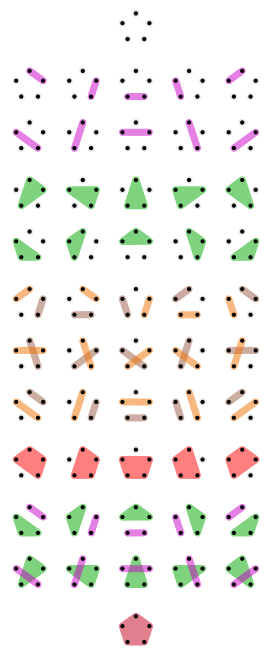
\includegraphics[scale=0.7]{./img/part.png}
\caption{\label{part} The 52 partitions of a set of 5 elements (source: wikipedia)}
\end{center}
\end{figure}

Now, if we consider ordered partitions, the jump appears earlier. The third ordered Bell number is thirteen and the fourth ordered Bell number is seventy-five\footnote{$75=5\times 15$ }. Moreover, in this case, all configurations are problematic, since they represent either coalitions or unbalanced power relations between elements. With this model, RAW and Korzybski's deduction appears earlier than they formulated it in term of number elements; four elements becoming the new tipping point.


\section*{The Law of Fives and the separation of powers}

When expressing the necessary bases for true democracy, John Locke and Montesquieu identify the need for the separation of powers (i.e. absence of coalition between powers) for \textit{representative democracy} in their respective essays \textit{Two Treatises of Government} \cite{Locke1689} and \textit{De l'esprit des lois} \cite{Montesquieu1748}. Moreover, modern criticisms of their work, when it comes to establish democracy, are aimed first at the fact that the organizations proposed respectively by Locke and Montesquieu do not provide a real separation of the powers but rather an interlocking of the powers; and second at the fact that the different powers identified are not put on an equal footing, some being more important than others.\\

Montesquieu identifies three powers \cite{Montesquieu1748}, that are now represented by different institutions in many representative democracies following the \textit{Age of Enlightenment}:
\begin{itemize}
\item the legislative power,
\item the executive power,
\item the judicial power.
\end{itemize}
In this setting with three powers, the third Bell number tells us that the number of possible coalitions (and therefore absence of true separation of powers) is four ($B_3 - 1$), and the third ordered Bell number tells us that number of possible coalitions or unbalanced power relations (and therefore absence of true separation of powers or equality between powers) is thirteen ($a_3$).\\
In other words, with both models, we obtain a number of possible relationships which the brain, the institutions, and people can handle.
It would therefore be theoretically possible to obtain true democracy with representative democracy.\\

However, new powers have been identified since, in particular:
\begin{itemize}
\item the mediatic power (also called ``the fourth power'') \cite{Bourdieu1996, Herman1988},
\item the economic power (also called ``the fifth power'') \cite{Ramonet1989, Ramonet1996}.
\end{itemize}
Adding these two powers changes the setting drastically. Having five powers means that the number of possible coalitions is given by the fifth Bell number, that is to say fifty-one ($B_5 -1$), and the number of possible coalitions or unbalanced power relations is five hundred and forty-one ($a_5$).\\
This situation becomes alarming because on top of not having institutions to help the separation of these new powers with the others (since the institutions have been created before their identification), the number of possible coalitions and unbalanced power relations becomes way too taxing for the brain, the institutions, and people to handle. Moreover, this issue can only get much worse the more powers are identified (we could, for instance, add Internet and public opinion\footnote{$B_6 = 203$ and $a_6 = 4683$.}) with jumps always getting larger.\\

\section*{Conclusion}

For these reasons, I would conclude that separation of powers is not enough of a base for true democracy. Consequently, representative democracies are not a viable political systems since it can not prevent a reign of power(s) and only encourages new aristocracies of greyfaces and totalitarianism. 
I would therefore encourage members of \textsc{The House of the Rising Collapse} to launch an \textit{Erisian Movement for Dysnomia, Daughter of Goddess} with a main focus on a total dissolution of all form of power and a direct democracy.

\begin{center}
\textit{Don't let them immanentize the eschaton!\\}

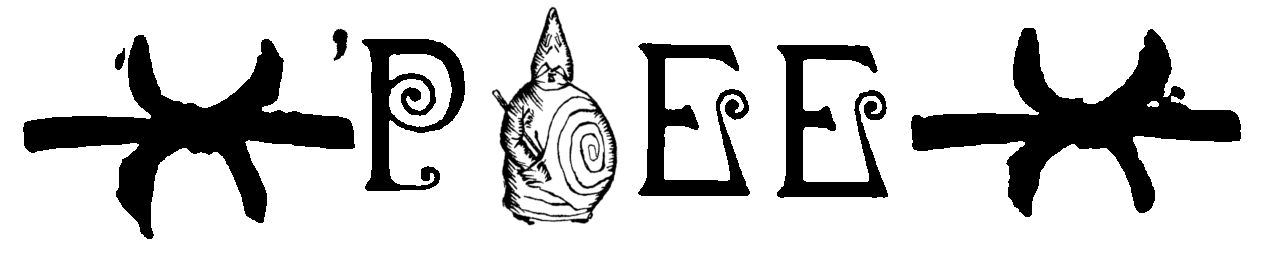
\includegraphics[scale=0.3]{./img/poee.png}
\end{center}

\section*{Acknowledgements}
This article has been written for the Patafizikhood of Eris Esoteric. It has NOT been conducted with the support of the AISB. Consult your pineal gland. \textsc{All Hail Discordia!!!!!}

%References
\bibliographystyle{unsrt}
\bibliography{coalitions_biblio}

\chapter{Why I am not an anarchist}
\chapterauthor{Gregory Hill}

\emph{This article was first published in No Governor, Vol. I, No. 2, 1975.\\}

About five years ago I considered myself an anarchist (anarchopacifist, in particular), because I believe that the highest authority available to any individual is one's own honest experience and that any other authority provides only vicarious information at best.\\
I've not changed my opinion about this, but I have ceased referring to myself as an anarchist. The reason is basic and simple: \textsc{too damn many rules}.\\
OK, it's a joke. But it's a \textsc{true} joke. The incompatibility is not between my position and some anarchist theories, but between my position and the position of most of those who use the label ``anarchist."\\
It seems that Rule Number One of anarchy, as understood by authoritarians and by most who call themselves anarchists, is that a government is an enemy. Rule Number Two is that to gain freedom the individual is politically or morally or somehow obligated to fight this enemy.\\
In my opinion, these rules represent a position which would be better referred to as anti-archy. The prefix ``a" means ``without" and it need not imply ``against". There is an exact parallel with the word atheist --- it is usually used and understood, by those for it and against it, as though the word was anti-theist.\\
I can respect the anti-archist position, but I don't share it. The government is not my enemy because there is no government. OK, another joke, but still a \textsc{true} joke. I know good and well that there are people with guns who restrict my free decisions, and I know about groups of people collecting taxes from me, and all the rest of this government business perceive it in the same manner that I perceive (for example) a big rock in my path which necessitates stepping around and compromising myself. Frankly, I don't believe in rocks either --- I just step around and compromise (which is actually easier than is believing in them). I think that there is a big difference in degree between (a) existentially responding to a phenomenon and (b) conceptualizing it as an ``enemy." If everything in the universe that has ever thwarted my purpose is my enemy, the only nothing can be my friend --- and that excludes even myself. But, still, I respect the anti-archist position. After all, if one does perceive a phenomenon to be an enemy then one would be a damn fool to do other than defend oneself.\\
Much of this essay is futzing around with labels. Still, I feel free to futz, and in any case what I'm trying to do is to avoid the assumption by others that I am at war with certain people just because those people think that they are a government and go out of their way to forcibly impose their notions on me.\\
I'm not at war with them or with rocks either. And insofar as anyone thinks that an anarchist is one who is supposed to do something or another, the there are too damn many rules for me ant to hell with the whole business.

\chapter{Stop the Rise of Insignificance}
\chapterauthor{Cornelius Castoriadis}

\emph{This text comes from an interview by Daniel Mermet for the radio program ``L\`a-bas si j'y suis" from 1996. Translated from French by Griffensteed the 5$^\text{lth}$.\\}

What characterizes the contemporary world are, of course, crises, contradictions, oppositions, fractures, but what strikes me the most is insignificance. Let us consider the feud between the right wing and the left wing. It has lost its meaning. Both of them say the same thing. Since 1983, the French socialists conducted a policy, then Mr. Balladur conducted the same policy; the socialists came back, they conducted, with Pierre Bérégovoy, the same policy; Mr. Balladur came back, he conducted the same policy; Mr. Chirac won the 1995 election saying "I'm going to do something else" and he conducted the same policy.\\
Political leaders are powerless. The only thing they can do is to go with the flow, which is to apply the trendy ultraliberal policy. The Socialists did no other thing once they returned to power. They are not political people, but politicians in the sense of micro-politicians. People who hunt votes by any means. They have no program. Their goal is to stay in power or return to power, and for that they are capable of anything.\\
There is an intrinsic link between this kind of nullity of politics, this becoming null of politics and this insignificance in other fields, in the arts, in philosophy or in literature. That is the spirit of the times. Everything conspires to extend insignificance.\\
Politics is a strange profession. Because it presupposes two skills that have no intrinsic relationship. The first is to gain power. If you don't come to power, you can have the best ideas in the world, it's useless; which implies an art of coming to power. The second ability is, once you're in power, to know how to govern.\\
There is no guarantee that someone who knows how to govern will be able to gain power. In the absolute monarchy, to gain power it was necessary to flatter the king, to be in the good graces of Madame de Pompadour. Today in our ``pseudo-democracy", coming to power means being telegenic, sensing public opinion.\\
I say ``pseudo-democracy" because I have always thought that the so-called representative democracy is not a true democracy. Jean-Jacques Rousseau had already said it: the English believe they are free because they elect representatives every five years, but they are free one day per five years, election day, that's all. Not that the election is rigged, not that they cheat in the polls. It's rigged because the options are set in advance. No one has asked the people what they want to vote on. We say to them: ``Vote for or against Maastricht". But who did Maastricht? It is not the people who made this treaty.\\
There is this wonderful phrase from Aristotle: ``Who is a citizen? A citizen is someone who is able to govern and be governed." There are millions of citizens in France. Why shouldn't they be able to govern? Because all political life aims precisely to make them unlearn it, to convince them that there are experts to whom to entrust business. So there is political counter-education. While people should get used to exercising all kinds of responsibilities and taking initiatives, they get used to following or voting for options that others present to them. And since people are far from  being stupid, the result is that they believe less and less and become cynical.\\
In modern societies, from the American revolution (1776) and the French revolution (1789) to the Second World War (1945), there was a thriving social and political conflict. People were opposed, demonstrated for political causes. The workers went on strike, and not always for small corporate interests. There were big questions that concerned all employees. These struggles have marked the last two centuries.\\
We are witnessing a decline in people's activity. It's a vicious circle. The more people withdraw from the activity, the more a few bureaucrats, politicians, supposedly responsible, take the lead. They have a good justification: ``I take the initiative because people do nothing." And the more they dominate, the more people say, ``It's no use getting involved, there's enough of them, and even then, we can't do anything about it anyway."\\
The second reason, related to the first, is the dissolution of the great political ideologies, either revolutionary or reformist, which really wanted to change things in society. For a thousand and one reasons, these ideologies have been discredited, have ceased to correspond to aspirations, to the situation of society, to historical experience. There was the massive event of the collapse of the USSR and communism in 1991. Has one person among the politicians --- not to say the schemers --- on the left, really thought about what happened? Why did this happen and who, as we say, has learned from it? While an evolution of this type, in its first phase --- the attainment of monstrosity, totalitarianism, the Gulag, etc. --- and then in the collapse, deserved a very thorough reflection and a conclusion on what a movement that wants to change society can do, must do, must not do, cannot do. Nothing!\\
And what do many intellectuals do? They brought out the strict liberalism of the early 19th century, that we fought for 150 years, and which would have led society to catastrophe. Because, in the end, the old Marx wasn't entirely wrong. If capitalism had been left to its own devices, it would have collapsed a hundred times. There would have been an overproduction crisis every year. Why didn't it collapse? Because workers fought, imposed wage increases, created huge internal consumer markets. They imposed reductions in working time, which absorbed all the technological unemployment. Now we are surprised that there is unemployment. But since 1940 working time hasn't decreased.\\
The Liberals tell us, "You have to trust the market." But academic economists themselves refuted this as early as the 1930s. These economists were not revolutionaries, nor were they Marxists! They have shown that all that the Liberals are saying about the virtues of the market, which would guarantee the best possible allocation of resources, the most equitable distribution of income, is absolute nonsense! All this has been demonstrated. But there is this great economic-political offensive of the governing and dominant layers that can be symbolized by the names of Mr. Reagan and Mrs. Thatcher, and even François Mitterrand! He said, "Okay, you've had enough fun. Now we'll fire you," we'll eradicate the "bad fat," as Mr. Juppé said. "And then you'll see that the market, in the long run, guarantees your well-being." In the long run. Meanwhile, there's 12.5\% official unemployment in France!

\section*{The Crisis is not a Fatality}

There has been talk of a kind of one-track thinking terrorism, that is, a non-thinking terrorism. It is one-track in the sense that it is the first thought that is an integral non-thought. A unique liberal thought that no one dares to oppose. What was Liberal ideology in its heyday? Around 1850, it was a great ideology because we believed in progress. Those Liberals thought that with progress there would be an increase in economic well-being. Even when we did not get richer, in the exploited classes, we went towards less workload, towards less arduous work: this was the great theme of the time. Benjamin Constant said: "Workers can't vote because they're dumbfounded by the industry [he says it bluntly, people were honest at the time!], so you need a census suffrage."\\
Afterwards, the working time decreased, there was literacy, education, a kind of Enlightenment that is no longer the subversive Enlightenment of the 18th century, but Enlightenment that spreads throughout society. Science develops, humanity becomes human, societies become more civilized, and little by little we will arrive at a society where there will be practically no more exploitation, where this representative democracy will tend to become a true democracy.\\
But it didn't work! So people no longer believe that idea. Today what dominates is resignation, even among the representatives of liberalism. What's the big argument right now? ``It may be bad, but the other alternative term was worse." And it's true that it frightened people a lot. They say to themselves, ``If we move too much, we go to a new Gulag." That is what is behind this ideological exhaustion and we will only come out of it if there really is a resurgence of a powerful criticism of the system. And a renaissance of people's activity, people's participation.\\
Here and there, we begin to understand that the ``crisis" is not a fatality of modernity to which we would have to subject ourselves, ``to adapt'' under penalty of archaism. We feel a shiver of renewed civic activity. Then the problem arises of the role of citizens and the competence of each to exercise democratic rights and duties with the aim --- sweet and beautiful utopia --- of getting out of generalized conformism.\\
To get out of it, should we be inspired by Athenian democracy? Who was elected in Athens? They didn't elect magistrates. They were designated by a random draw or by rotation. For Aristotle, remember, a citizen is one who is capable of governing and being governed. Everyone is capable of governing, so we do random draws. Politics is not a matter for specialists. There is no political science. There's an opinion, the Greek doxa, there's no episteme\footnote{Theoretically founded knowledge, science.}.\\
The idea that there is no polics expert and that all opinions are equal is the only reasonable justification for the majority principle. Thus, among the Greeks, the people decide and the magistrates are designated randomly or by rotation. For specialized activities --- shipyard construction, temple construction, warfare --- specialists are needed. Them, they do get elected. That is election. Election means ``choice of the best". Here is where education of the people comes in. We do a first election, we're wrong, we find that, for example, Pericles is a deplorable strategist, well, we don't re-elect him or we revoke him.\\
But the doxa must be cultivated. And how can a doxa be cultivated for the government? By governing. Therefore democracy --- it is important --- is a matter of educating citizens, which does not exist at all today.

\section*{``Rest or Be Free"}

Recently, a journal published a statistic indicating that 60\% of MPs, in France, admit they understand nothing about the economy. MPs who decide all the time! In truth, these members, like ministers, are subjugated to their technicians. They have their experts, but they also have prejudices or preferences. If you follow closely the functioning of a government, of a large bureaucracy, you see that those who lead rely on experts, but choose among them those who share their opinions. It's a completely stupid game and that's how we're governed.\\
Today's institutions repel, distance and dissuade people from participating in business. While the best education in politics is active participation, which implies institutional transformation that enables and encourages that participation.\\
Education should be much more focused on the common thing. We should understand the mechanisms of the economy, society, politics, etc. Children get bored learning history when it's fascinating. We should teach a true anatomy of contemporary society, how it is, how it works. Learn to defend beliefs, ideologies.\\
Aristotle said, "Man is an animal that desires to know." That is not true. Man is an animal that desires belief, that desires the certainty of belief, hence the hold of religions, of political ideologies. In the labour movement, at first, there was a very critical attitude. Take the second verse of The International, the song of Paris Commune: ``There is no Supreme Savior, no God --- exit religion --- no Caesar, no tribune" --- exit Lenin!\\
Today, even if a minority still seeks faith, people have become much more critical. This is very important. Scientology, sects, or fundamentalism, it's in other countries, not here, not so much. People have become much more skeptical. Which also hinders their will to act.\\
Pericles in the speech to the Athenians said: ``We are the only ones in whom reflection does not inhibit action." That's admirable! He adds: ``The others, either they do not think and they are reckless, they commit absurdities, or, by thinking, they don't manage to do anything because they say to themselves, there is discourse and there is the opposite discourse''. Right now, we're definitely going through an inhibition phase. Once bitten, twice shy. We don't need big speeches, we need true speeches.\\
Anyway, there is an irreducible desire. If you take archaic societies or traditional societies, there is not an irreducible desire, a desire such as it is transformed by socialization. These societies are societies of repetition. For example, we say: ``You will take a woman from such a clan or from such a family. You'll have a wife in your life. If you have two, or two men, it'll be secret, it'll be a transgression. You'll have a social status, it'll be that and nothing else."\\
Today, however, there is a liberation, in every sense of the word, from the constraints of the socialization of individuals. We have entered an age of unlimitedness in all fields, and it is due to this that we have the desire for infinity. This liberation is in a sense a great conquest. There is no question of returning to societies of repetition. But we must also --- and this is a very great theme-- learn to limit ourselves, individually and collectively. The capitalist society is a society that runs into the abyss, from every point of view, because it does not know how to limit itself. And a truly free society, an autonomous society, has to know how to limit itself, how to know that there are things you can't do or even try to do or want.\\
We live on this planet that we are destroying, and when I say this sentence I think of the wonders, I think of the Aegean Sea, I think of the snow-covered mountains, I think of the view of the Pacific from a corner of Australia, I think of Bali, India, the French countryside that is being desertified. So many wonders in the process of demolition. I think we should be the gardeners of this planet. It should be cultivated. Grow it as it is and for itself. And find our life, our place in it. That is a huge task. And it could absorb a large part of people's leisure time, freed from a stupid, productive, repetitive work, etc. This is not only far away from the current system but also from the current dominant imagination. The imagination of our time is that of unlimited expansion, the accumulation of junk --- a TV in every room, a microcomputer in every room ---, that is what we must destroy. The system relies on that imagination.\\
Freedom is very difficult. Because it's very easy to let yourself go. Man is a lazy animal. There's a wonderful phrase from Thucydides: ``You have to choose: rest or be free." And Pericles said to the Athenians, ``If you want to be free, you must work." You can't rest now. You can't sit in front of the TV. You're not free when you're watching TV. You think you are free by flicking through channels like an idiot, you are not free, it is a false freedom. Freedom is activity. And freedom is an activity that at the same time limits itself, that is, it knows that it can do everything but that it must not do everything. That is the great problem of democracy and individualism.




\chapter{Manifesto}
\chapterauthor{John Cage}

\emph{The text below was written for Julian Beck and Judith Malina, directors of the Living Theatre, for use in their program booklet when they were performing at the Cherry Lane Theatre, Greenwich Village, New York.\\}

\vspace{2cm}
\hspace{-2.5cm}
\setlength{\tabcolsep}{1pt}
\begin{tabular}{l l c}
$\left.\begin{tabular}{l}
written in response\\
to a request for\\
a manifesto on\\
music, 1952
\end{tabular}\right\}$
& instantaneous & and unpredictable\\

& $\left.\begin{tabular}{l}
\begin{tabular}{c c c c c c c c c}
nothing & is & accomplished & by & writing & a & piece & of & music\\
" & " & " & " & hearing & " & " & " & "\\
" & " & " & " & playing & " & " & " & "\\
\end{tabular}
\end{tabular}\right\}$
& \begin{tabular}{c}
our ears are\\
now\\
in excellent condition
\end{tabular}
\end{tabular}

\end{document}


















